\documentclass[11pt]{article}
\usepackage{classTools}

\begin{document}

% To include a problem set header, use the psHeader command
\psHeader{1}{Wed Sep. 14, 2022 (11:59pm)}

Please review the Syllabus for information on the collaboration policy, grading scale, revisions, and late days.


\begin{enumerate}
    \item (Asymptotic Notation) 
    \begin{enumerate}
    \item (practice using asymptotic notation)
        Fill in the table below with ``T'' (for True) or ``F'' (for False) to indicate the relationship between $f$ and $g$. For example, if $f$ is $O(g)$, the first cell of the row should be ``T.'' \\
        \begin{table}[h!]
        \centering
        \bgroup
        \def\arraystretch{1.3}
        \begin{tabular}{||c | c || c | c | c | c | c ||}
         \hline
         $f$ & $g$ & $O$ & $o$ & $\Omega$ & $\omega$ & $\Theta$ \\
         \hline\hline
         $\sqrt{n}$ & $\log n$ & F & F & T & T & F  \\ \hline
         $n^{\sqrt{n}}$ & $n^{\log n}$ & F & F & T & T & F \\ \hline
         $(\log {n^{120}})^2\sqrt{n}$ & $n$ & T & T & F & F & F \\ \hline
         $\log(2^n)$ & $\log(e^n)$ & T & F & T & F & T \\ \hline
         $2^{\sqrt{n}}$ & $n^{\log n}$ & F & F & T & T & F \\ \hline
         $n^{(n \bmod 2)}$ & $n^{1/3}$ & F & F & F & F & F \\ \hline
        \end{tabular}
        \egroup
        \end{table}
        Recall that, through CS120, all logarithms are base 2 unless otherwise specified. 
        
    \item  (rigorously reasoning about asymptotic notation)  
    For each of the following claims, either justify why the statement holds (for all $f$, $g$) or provide a counterexample. In all cases, take the domain of the functions $f$ and $g$ to be the natural numbers (rather than the positive reals), and assume $f(n), g(n)\geq 1$ for all sufficiently large $n$.
    \begin{itemize}
        \item For all positive constants $a$ and $b$, if $f(n) = \Theta(a^n)$ and $g(n) = \Theta(n^b)$, then $f(g(n)) = \Theta(a^{(n^b)})$.

\begin{proof}
This is not true. Assume $f(n) = a^n$ and $g(n) = 2n^b$. Then $f(g(n)) = (a)^{(2n^b)} = (a^{(n^b)} )^2 \neq \Theta(a^{(n^b)})$.
\end{proof}

        \item For all positive constants $a$ and $b$, if $f(n) = \Theta(a^n)$ and $g(n) = \Theta(n^b)$, then $g(f(n)) = \Theta((a^n)^b)$.
        
\begin{proof}
This is true. We do have to prove this equality both ways, which is a little annoying. First considering big-$O$ notation, we have some $c_1, c_2 > 0$ such that $f(n) \leq c_1 a^n$ and $g(n) \leq c_2 n^b$ for $n$ large enough. Then because both of these functions are positive and increasing, the inequality is preserved under function composition: $g(f(n)) \leq c_2 (c_1 a^n) ^b = c_2 c_1^b (a^n)^b = \Theta ((a^n)^b)$. \\

Next, we handle the $\Omega$ case. We assign $d_1, d_2 > 0$ so $f(n) \geq d_1 a^n$ and $g(n) \geq d_2 n^b$ for $n$ large enough. Then the inequality is preserved again when we compose functions: $g(f(n)) \geq c_2 (c_1 a^n) ^b = c_2 c_1^b (a^n)^b = \Theta ((a^n)^b)$. \\

Because we showed that this was true for both big-$O$ and big-$\Omega$, we can say that $g(f(n)) = \Theta((a^n)^b)$.
\end{proof}

    \end{itemize}
  
    \end{enumerate}
    
    \newpage
    
    \item (Understanding computational problems and mathematical notation)\\\\
    Recall the definition of a {\em computational problem} from Lecture Notes 1.  

 
    Consider the following computational problem $\Pi=(\Inputs,\Outputs,f)$ and algorithm $\BC$ to solve it, where
    \begin{itemize}                                
    \item $\Inputs = \N\times\N\times \N$ 
    \item $\Outputs = \{(c_0,c_1,\ldots,c_{k-1}) : k,c_0,\ldots,c_{k-1}\in \N\}$
    \item $f(n,b,k) = \{ (c_0,c_1,\ldots,c_{k-1}) : n=c_0+c_1b+c_2b^2+\cdots+c_{k-1}b^{k-1}, \forall i\ 0\leq c_i< b\}.$ 
    \end{itemize}

    
\begin{algorithm}[H]
    \BC{$n,b,k$}\\
    {
%    \Input{$(n,b)$}
%    \Output{$(k,(c_0,c_1,\ldots,c_{k-1}))$}
    \lIf{$b<2$}{\Return{$\bot$}}
    \ForEach{$i=0,\ldots,k-1$}{
    $c_i = n \bmod b$\;
    $n = (n-c_i)/b$\;
    }
    \lIf{$n==0$}{\Return{$(c_0,c_1,\ldots,c_{k-1})$}}
    \lElse{\Return{$\bot$}}}
\end{algorithm}


\begin{enumerate}
\item Describe the computational problem $\Pi$ in words.  (You may find it useful to try some examples with $b=10$.)
\item For each possible input $x\in \Inputs$, what is $|f(x)|$?  Justify your answers in one or two sentences.


\item This problem does not refer to $\Pi$ and instead refers to an abstract computational problem. A one- or two-sentence explanation for this the questions should suffice:
%\begin{enumerate}
%\item 

Let $\Pi=(\Inputs,\Outputs,f)$ and $\Pi'=(\Inputs,\Outputs,f')$ be two computational problems.  Suppose that for all $x\in \Inputs$, we have $f(x)\subseteq f'(x)$.  Does it follow that every algorithm $A$ that solves $\Pi$ also solves $\Pi'$?    Does the answer change if we also require that $f(x)\neq \emptyset$ for every $x$? Justify your answers with a proof or a counterexample.
%\end{enumerate}


\end{enumerate}

\begin{proof}
\begin{enumerate}

\item The problem takes in an integer $n$, a base system $b$, and a number of digits $d$. It returns the base $b$ representation of $n$ one digit at a time, up to $d$ digits, and does so backwards. It's entirely possible that we requested too many digits, and so then we would have a bunch of leading zeroes listed (or, because things go backwards, trailing zeroes). If the number of digits requested is too small to list every digit, the algorithm fails and returns $\bot$. Lastly, a ``digit" is entirely dependent on what the base system is - in binary, we only have 0 and 1, and we go 0 to $F$ in hexadecimal; any other system (in positive integers) is possible too.

\item $| f(x) |$ is either $k$ or $\bot$. We are guaranteed that an answer we return will have $k$ terms by the pseudocode; this happens when $x$ is expressible in base $b$ with fewer than or equal to $k$ digits. Otherwise, we return $\bot$ because we can't fully express $x$.

\item This does not follow - suppose $f, f'$ are the same function but $\Pi$ requires that we return $\bot$ when $n \neq 0$ at the end of our loop while $\Pi'$ does not. Then obviously the algorithm does not solve the second problem. If we remove the ability for $f(x) = \emptyset$, then $\Pi$ always returns some value in $\mathcal{O}$ (because it can never return $\bot$). Then $f(x), f'(x)$ both return something of the same size because their outputs are in $\mathcal{O}$. Since $f(x) \supseteq f' (x)$ and $| f(x) | = | f'(x) |$, $f(x) = f'(x)$ and so now the same algorithm $A$ solves both problems.

\end{enumerate}
\end{proof}

\newpage

\item (Radix Sort) In the Sender--Receiver Exercise on Thursday September 8, you studied the sorting algorithm {\em Counting Sort}, generalized to arrays of key--value pairs, and proved that it has running time $O(n+U)$ when the keys are drawn from a universe of size $U$. In this problem you'll study {\em Radix Sort}, which improves the dependence on the universe size $U$ from linear to logarithmic.  Specifically, Radix Sort can achieve runtime $O(n+n(\log U)/(\log n))$, so it achieves runtime $O(n)$ whenever $U = n^{O(1)}$.  
Radix Sort is constructed by using Counting Sort as a subroutine several times, but on a smaller universe size $b$.
Crucially, Radix Sort uses the fact that Counting Sort can be implemented in a way that is {\em stable} in the sense that it preserves the order in the input array when the same key appears multiple times.  Here is pseudocode for Radix Sort:

\begin{algorithm}[H]
\AreaofConvexPolygon{$U,b,A$}\\
\Input{A universe size $U\in \N$, a base $b\in \N$ with $b\geq 2$, and an array $A=((K_0,V_0),\ldots,(K_{n-1},V_{n-1}))$, where each $K_i\in [U]$}
\Output{A valid sorting of $A$}
%$b=\min\{n,U\}$\;
$k=\lceil (\log U)/(\log b)\rceil$\;
\ForEach{$i=0,\ldots,n-1$}{
    $V_i' = \BC(K_i,b,k)$}
\ForEach{$j=0,\ldots,k-1$}{
    \ForEach{$i=0,\ldots,n-1$}{
    $K'_i = V'_i[j]$
    }
    $((K_0',(V_0,V'_0)),\ldots,(K_{n-1}',(V_{n-1},V'_{n-1}))) = \CountingSort(b,((K'_0,(V_0,V_0')),\ldots,(K'_{n-1},(V_{n-1},V'_{n-1})))$\;
}
\ForEach{$i=0,\ldots,n-1$}{
    $K_i = V'_i[0]+V'_i[1]\cdot b + V'_i[2]\cdot b^2+\cdots+V'_i[k-1]\cdot b^{k-1}$}
\Return{$((K_0,V_0),\ldots,(K_{n-1},V_{n-1}))$}
\caption{Radix Sort}
\end{algorithm}

(You can also read a description of Radix Sort in CLRS Section 8.3 for the case of sorting arrays of keys (without attached items) when $U$ and $b$ are powers of 2, albeit using different notation than us.)

        \begin{enumerate}
        
            \item (proving correctness of algorithms) Prove the correctness of \RadixSort\ (i.e. that it correctly solves the Sorting problem).  Where does your proof use the stability of \CountingSort?
      
            
            \item (analyzing runtime) Show that \RadixSort\ has runtime $O((n+b)\cdot \lceil \log_b U\rceil)$.  Set $b=\min\{n,U\}$ to obtain our desired runtime of $O(n+n(\log U)/(\log n))$.  (This runtime analysis is outlined in CLRS, but you'd need to adapt it to our notation and slightly more general setting.) 
            
            \item (implementing algorithms)
            Implement \RadixSort\ using the implementations of \CountingSort\ and \BC\ that we provide you in the GitHub repository. 
  
 \iffalse           
            Provide a more detailed pseudocode description of Radix Sort (for arrays of item-key pairs) following the above outline, using Counting Sort as a subroutine.  The inputs to Counting Sort are a natural number $U$ and an array $A$ of item-key pairs where the items are arbitrary objects and the keys are elements of $[U]$, so for each call your pseudocode makes to Counting Sort,  it should explicitly say what value of $U$ and what array $A$ is fed in. 
            Implement your version of Radix Sort in Python, using the implementation of Counting Sort that we will provide you in the github repository.
                The inputs to your implementation of Radix Sort should consist of an array of item-key pairs, the length $n$ of the array, the universe size $U$, and the
                base $b$.
\fi

            \item (experimentally evaluating algorithms) Run experiments to compare the expected runtime of \CountingSort, \RadixSort (with base $b=n$), and \MergeSort\ as $n$ and $U$ vary among powers of 2 with $1\leq n\leq 2^{16}$ and $1\leq U\leq 2^{20}$.  For each pair of $(n,U)$ values you consider, run multiple trials to estimate the expected runtime over random arrays where the keys are chosen uniformly and independently from $[U]$.  For each sufficiently large value of $n$, the asymptotic (albeit worst-case) runtime analyses suggest that \CountingSort\ should be the most efficient algorithm for small values of $U$, \MergeSort\ should be the most efficient algorithm for large values of $U$, and \RadixSort\ should be the most efficient somewhere in between.  Plot the transition points from \CountingSort to \RadixSort, and \RadixSort to \MergeSort\ on a $\log n$ vs. $\log U$ scale (as usual our logarithms are base 2).  Do the shapes of the resulting transition curves fit what you'd expect from the asymptotic theory?  Explain.  %(Note: depending on your implementation and your computer, the experiments may take hours, so be sure to carry them out well ahead of the deadline.)
            
            \textit{Note: We are expecting to see one (or more, if necessary) graphs that demonstrate, for every value of $n$, for which value of $U$ \RadixSort first outperforms \CountingSort and \MergeSort first outperforms \RadixSort. You should label the graphs appropriately (title, axis labels, etc.) and provide a caption, as well as an answer and explanation to the above question. Please look at the provided starter code for more information on generating random arrays, timing experiments, and graphing. Your implementation of RadixSort, as well as any code you write for experimentation and graphing need not be submitted.  Depending on your implementation, running the experiments could take anywhere from 15 minutes to a couple of hours, so don't leave them to the last minute!}   

          
        \end{enumerate}
        
\begin{proof}
\begin{enumerate}[label = (\alph*)]

\item We can do this by induction - if we can be convinced that in the $k^{th}$ step, the last $k$ digits of the numbers are sorted (so the first digits in their backwards-stored array), then when we are done, the numbers should be completely sorted correctly. Henceforth, we refer to numbers in the way that our BC algorithm spits them out - in base $b$ and reverse order. To begin, we note that the algorithm correctly sorts the first digits in our lists - this is the same as our \CountingSort algorithm on one digit numbers.

Now assume the first $k$ digits are correctly sorted. We look at the $(k + 1)^{th}$ digit and apply \CountingSort again. I claim that any two numbers after this will be correctly sorted. Suppose they have different $(k + 1)^{th}$ digits. Then the most recent digit sorted will dominate and since \CountingSort works, the two numbers will be correctly sorted. Now suppose these two numbers have the same $(k + 1)^{th}$ digit. The one with the smaller lower digits will have been closer to the front of the array of numbers to sort, so it will end up closer to the front of the linked list relating to the $(k + 1)^{th}$ digit that the two numbers share. Therefore the correct ordering is still preserved, and we are done. \RadixSort works.

\item We run three sets of operations which we need to examine for runtime - lines 3-4, 5-8, and 9-10 in the pseudocode. In lines 3-4, we do the \BC operation $n$ times. When we do the \BC operation, it creates $\lceil \log_b U \rceil$ digits by doing division and subtraction that many times; therefore the runtime of this step is the product of these two results.

In lines 5-8, we assign a value $K_i '$ $n$ times, which has a runtime of $n$, and then do \CountingSort $k = \lceil \log_b U \rceil$ times. We discussed in class that the runtime of \CountingSort is $O(n + U)$, where $U$ is in particular the size of the universe over which we distribute our key-value pairs. In this case, we only need to distribute out over each of the $b$ possible digits! Therefore our counting sort runtime is $O((n + b) \cdot \lceil \log_b U \rceil)$.

In lines 9-10, we carry out $n$ iterations of $O(k) = O(\lceil \log_b U \rceil)$ operations.

Now we can add these up:

$$
O(n \cdot \lceil \log_b U \rceil + (n + b) \cdot \lceil \log_b U \rceil + n \cdot \lceil \log_b U \rceil) = O((n + b) \cdot \lceil \log_b U \rceil),
$$

as desired. It is not difficult to see that if we use $b = \min \{ n, U \}$ we get to our final answer: if $n \leq U, O((n + b) \cdot \lceil \log_b U \rceil) = O((n + n) \cdot \lceil \log_n U \rceil) = O((n + n) \cdot \log U / \log n)$. As $U \geq n$, we can see that $O((n + n) \cdot \log U / \log n) = O(n \cdot \log U / \log n + n \cdot \log U / \log n) = O( n + n  \cdot \log U / \log n)$. Now suppose $U < n$. THen our expression is $O((n + U) \cdot \lceil \log_U U \rceil) = O(n + U)$. As we know again that $U < n \cdot  \log U / \log n$, we are done.

\item

See code.

\item 

See the chart below.

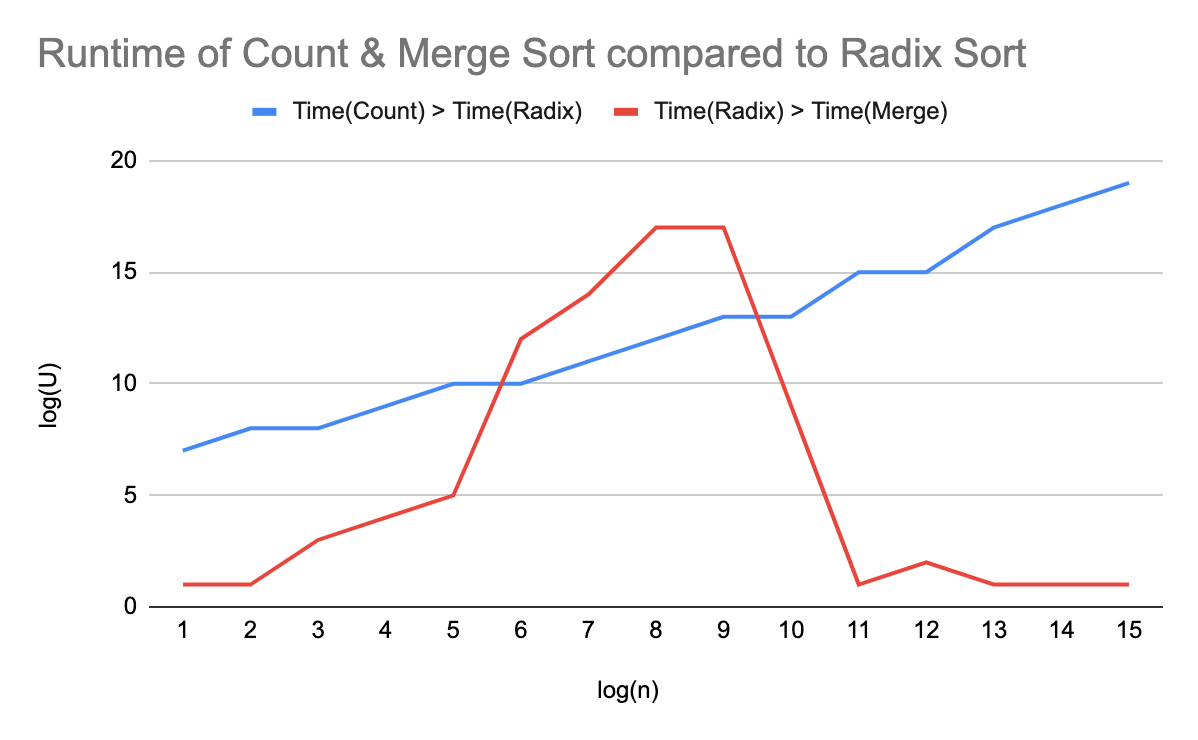
\includegraphics[width = 5in]{1-1}

This graph shows the smallest value of $U$ for which we find the runtime for \MergeSort to be less than \RadixSort (in red), and the smallest value for which we find the runtime of \RadixSort to be less than \CountingSort (in blue). This is carried out for all positives integer powers of 2 up to $2^{15}$. We expected to see that \MergeSort is most effective when $U$ is large, which is in fact what we see here - above the values of $\log(n) = 9, 10$, the graph plummets. We also see that the point at which \RadixSort outperforms \CountingSort climbs pretty linearly with $\log (n)$. This in general comports with what I expect - \MergeSort fails when it has to deal with too many data points and becomes slow; \CountingSort fails
\end{enumerate}
\end{proof}

\end{enumerate}


\end{document}